\documentclass[conference,a4paper]{IEEEtran}
\IEEEoverridecommandlockouts
\usepackage{cite}
\usepackage{amsmath,amssymb,amsfonts}
\usepackage{graphicx}
\usepackage{textcomp}
\usepackage{array}
\usepackage{url}
% Ragged-right paragraph column whose width is a fraction of the column.
\newcolumntype{P}[1]{>{\raggedright\arraybackslash}p{\dimexpr#1\columnwidth-2\tabcolsep\relax}}
% Forces the second row of the six-author block (IEEEtran has no command).
\makeatletter
\newcommand{\linebreakand}{%
  \end{@IEEEauthorhalign}
  \hfill\mbox{}\par
  \mbox{}\hfill\begin{@IEEEauthorhalign}
}
\makeatother

\begin{document}

\title{Calibrated Escalation for IT Ticket Triage: What the Calibration Distribution Decides}

\author{\IEEEauthorblockN{Aryan Waingankar}
\IEEEauthorblockA{\small\textit{Symbiosis Institute of Technology, Pune}\\
\small India\\
\footnotesize aryan.waingankar.btech2023@sitpune.edu.in}
\and
\IEEEauthorblockN{Shreyansh Pandey}
\IEEEauthorblockA{\small\textit{Symbiosis Institute of Technology, Pune}\\
\small India\\
\footnotesize shreyansh.pandey.btech2023@sitpune.edu.in}
\and
\IEEEauthorblockN{Parth Bagle}
\IEEEauthorblockA{\small\textit{Symbiosis Institute of Technology, Pune}\\
\small India\\
\footnotesize parth.bagle.btech2023@sitpune.edu.in}
\linebreakand
\IEEEauthorblockN{Swapnil Samrat}
\IEEEauthorblockA{\small\textit{Symbiosis Institute of Technology, Pune}\\
\small India\\
\footnotesize swapnil.samrat.btech2023@sitpune.edu.in}
\and
\IEEEauthorblockN{Madhvi Saxena}
\IEEEauthorblockA{\small\textit{Symbiosis Institute of Technology, Pune}\\
\small India\\
\footnotesize madhvi.saxena@sitpune.edu.in}
\and
\IEEEauthorblockN{Aditi Saxena}
\IEEEauthorblockA{\small\textit{Symbiosis Institute of Technology, Pune}\\
\small India\\
\footnotesize aditi.saxena@sitpune.edu.in}}

\maketitle

\begin{abstract}
A triage system for IT support tickets must route each ticket to the right team and recognise when to hand it to a person. Our pipeline has two separately calibrated escalation gates: a 0.50 confidence threshold on a fast lexical classifier decides whether a slower embedding classifier is consulted, and a 0.67 cosine-similarity threshold on retrieved past tickets decides whether a language model may draft a resolution. On a 9-ticket adversarial set the retrieval gate decides every ticket correctly, against 3 of 9 without it. A zero-shot LLM classifies more accurately (40/45 against 33/45) but cannot abstain. On 108 tickets written and cross-labelled by two authors ($\kappa$ = 0.936), the cascade routes 74 of 98 correctly, but the gate also escalates 32 actionable tickets. On 583 distinct real tickets covering two of seven teams, it routes 19.7\% correctly (50.4\% under an alternative mapping), and 371 of 468 misrouted tickets reach the drafter: a classifier trained only on synthetic templates does not transfer to real tickets, and the data a component is trained or calibrated on limits it more than the method chosen. Conclusions are scoped to small evaluation sets.
\end{abstract}

\begin{IEEEkeywords}
IT ticket triage, selective prediction, escalation, calibration, conformal prediction, retrieval-augmented generation
\end{IEEEkeywords}

\section{Introduction}\label{sec:intro}

A triage system that routes a ticket confidently but wrongly costs more than one that asks for help, so when it declines to answer matters as much as its accuracy. In our pipeline escalation to a human is a first-class output: a two-tier cascade assigns one of seven teams, similar resolved tickets are retrieved, and a language model may draft a resolution only when the closest past ticket is similar enough. Both thresholds come from measured calibration data (Section~\ref{sec:thr}), and a zero-shot LLM, more accurate but unable to abstain (Section~\ref{sec:zs}), is kept as a baseline. The contributions are:

\begin{itemize}
\item \textbf{A two-gate escalation pipeline} whose thresholds are calibrated independently, with the evidence for each value and the calibration attempts we rejected.
\item \textbf{A recurring finding:} the data distribution used to fit or calibrate a component constrains it more than the method or test applied to it.
\item \textbf{Transparent baselines and error analysis:} a controlled ablation, zero-shot LLM baselines from two vendors, an audit of an LLM judge, and a breakdown of misclassifications, wrong escalations and unsupported drafts.
\item \textbf{An extended evaluation} on 108 tickets written and cross-labelled by two authors ($\kappa$ = 0.936) and 583 real tickets from a public dataset, reported with its negative result.
\end{itemize}

\section{Related Work}\label{sec:rw}

LLM-based methods route and escalate IT and customer-support tickets \cite{b1,b2,b3} and mainly report routing accuracy; our focus is the decision to abstain. Confidence-based cascades pass difficult inputs to a more capable model \cite{b4}, conformal variants give distribution-free guarantees for multi-tier cascades \cite{b5}, and a cascade can end with a human \cite{b6}. Split conformal prediction guarantees marginal coverage under exchangeability \cite{b7}, \cite{b8}; weighted conformal prediction restores it under covariate shift when the likelihood ratio is known \cite{b9}, and later work bounds the loss when exchangeability fails \cite{b10} and adapts online \cite{b11}; our shift is a change in writing style. A retrieval-augmented generation (RAG) system \cite{b12} can abstain when the retrieved context is insufficient \cite{b13} or correct itself when retrieval is poor \cite{b14}. LLM judges can come with guaranteed human agreement \cite{b15} and show an agreeableness bias \cite{b16}. Synthetic data's value as a benchmark has been studied \cite{b17}. Table~\ref{tab:rel} compares the closest works using only their abstracts: two ticket-triage studies evaluate on real tickets, while our main evaluation is synthetic (Section~\ref{sec:ext}), and none combines gates calibrated on measured data with generation permitted only after retrieval passes such a gate. Confidence-based \cite{b4} and conformal \cite{b5} cascades set their thresholds on held-out in-distribution data, and split conformal guarantees \cite{b7}, \cite{b8} assume exchangeable calibration and test tickets; we choose and re-check each threshold on deliberately shifted sets (paraphrased, adversarial, human-written, real) and report where the guarantees fail (Section~\ref{sec:cov}).

\begin{table}[!t]
\caption{Comparison with the closest related work, based on each paper's abstract}\label{tab:rel}
\centering
\scriptsize
\setlength{\tabcolsep}{3pt}
\begin{tabular}{|P{0.210}|P{0.230}|P{0.280}|P{0.280}|}
\hline
\textbf{Work} & \textbf{Task} & \textbf{Abstention mechanism} & \textbf{Evaluated on}\\ \hline\hline
TickIt \cite{b1} & Ticket escalation & Routes tickets to support teams & Deployment on Volcano Engine\\ \hline
Paket et al. \cite{b2} & Service desk ticket classification & not stated & Turkish service desk tickets, 172 classes\\ \hline
Carroll et al. \cite{b3} & REDCap ticket triage and drafting & not stated & Real REDCap tickets, expert-rated\\ \hline
Jitkrittum et al. \cite{b4} & Cascade deferral & Confidence-based and post-hoc deferral & not stated\\ \hline
Conformal Cascade \cite{b5} & Multi-tier LLM inference & Defer unless conformal set is a singleton & Multiple-choice benchmarks\\ \hline
Fanconi et al. \cite{b6} & Human--AI decision-making & Deferral, then abstention to a human expert & General and medical QA\\ \hline
Sufficient context \cite{b13} & RAG error analysis & Sufficient-context guided abstention & Several models and datasets\\ \hline
CRAG \cite{b14} & Robust RAG & Retrieval evaluator triggers corrective actions & Short- and long-form generation\\ \hline
Ours & IT ticket triage & Two calibrated gates (confidence, retrieval) & Synthetic corpus; 45-ticket out-of-template set; 108 author-written; 583 real tickets\\ \hline
\end{tabular}
\end{table}

\section{Methodology}\label{sec:meth}

\subsection{Pipeline and gates}\label{sec:pipe}

Fig.~\ref{fig:pipe} shows the pipeline: sequential, with agent boundaries and an HTTP interface, not an autonomous multi-agent system. One orchestrator takes every routing decision and traces every stage, so a skipped resolution step is direct evidence that no language model was called; a failed stage escalates the ticket. Tier 1 is TF-IDF with logistic regression over a committed vocabulary; its label is accepted if its highest class probability is at least 0.50, and otherwise Tier 2, logistic regression over frozen BGE embeddings \cite{b18} (bge-base-en-v1.5, 768 dimensions), classifies the ticket. The five nearest resolved tickets are retrieved from a FAISS inner-product index \cite{b19}. Below a top-1 cosine similarity of 0.67 the ticket is escalated and no language model is called; otherwise Gemini (gemini-flash-lite) drafts a resolution based only on the retrieved resolutions, recommending a human check when they do not fit. The language model never assigns the category. The cascade threshold depends only on Tier-1 confidence, so the Tier-2 encoder can be replaced without recalibrating it; the retrieval threshold must be recalibrated with the encoder. Offline, resolved tickets are clustered by resolution-text similarity at 0.80 into automation candidates for a reviewer.

\begin{figure}[!t]
\centering
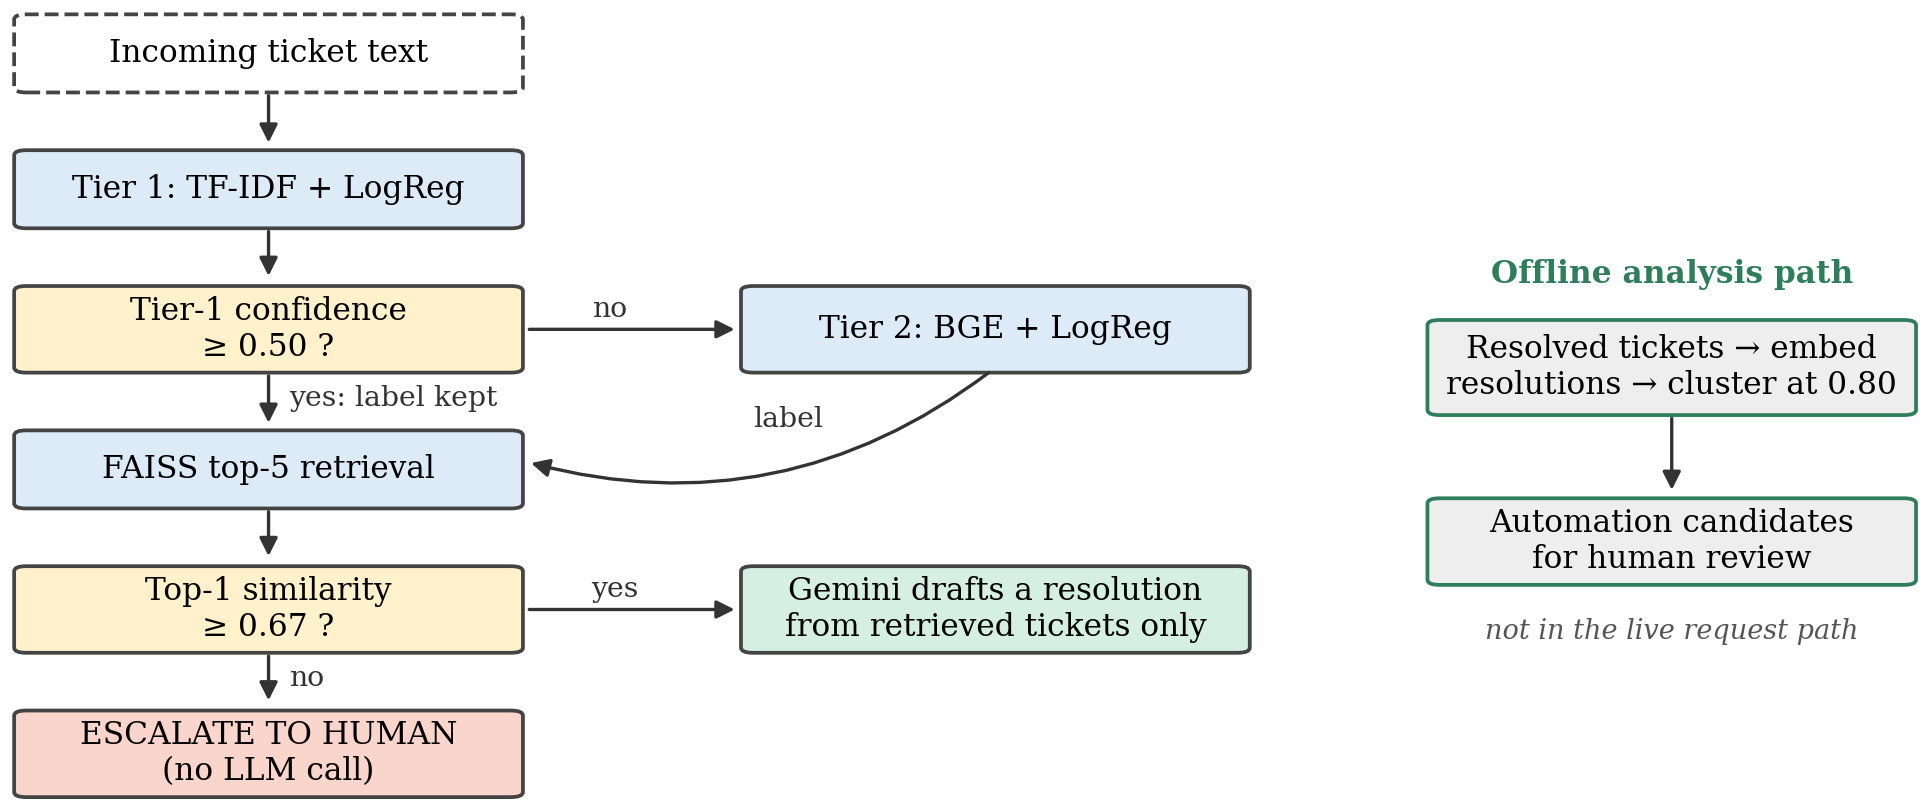
\includegraphics[width=3.3in]{fig1_pipeline.png}
\caption{The pipeline. Two separately calibrated gates decide escalation; the language model drafts only above the retrieval gate and never assigns the category. The offline path clusters resolved tickets into automation candidates.}\label{fig:pipe}
\end{figure}

\subsection{Conformal measurement and verification}\label{sec:conf}

To test whether a finite-sample guarantee could replace the cascade threshold, we calibrate split conformal prediction \cite{b7}, \cite{b8} for each tier on a held-out set; its prediction sets have marginal miscoverage at most $\alpha$ when calibration and test tickets are exchangeable. It runs offline and gates nothing. Automated checks (online supplement) run before any result is accepted: routing decisions are compared exactly, and floating-point values within tolerances derived from their arithmetic.

\section{Experimental Setup}\label{sec:setup}

\textbf{Dataset.} Following the nasscom use-case brief, which specified seven categories, routing, resolution suggestion, confidence-based escalation and automation flagging and recommended a synthetic, LLM-generated dataset, we generated 4,000 tickets (title, description, category, resolution, priority). The seven categories are Access Management, Application, Database, Infrastructure, Network, Security and Storage. The synthetic corpus, a requirement of the brief, limits what can be claimed (Section~\ref{sec:lim}): the generation templates coincide with the resolution classes, so clustering precision cannot be measured, and memorisation is template-level (the calibration set touches 62 of the 66 templates, and removing whole templates would leave 210 of the 4,000 rows), so the corpus cannot be decontaminated by filtering.

\textbf{Evaluation sets.} Held-out accuracy on generated data is uninformative (the TF-IDF baseline scores 100\%). Table~\ref{tab:splits} lists every split. Tier 2 and DistilBERT are trained on a stratified 3,200-row split (seed 42); the production Tier 1 is fitted on all 4,000 rows. Evaluation uses fixed, read-only sets written outside the templates: a hand-written 14-ticket benchmark, a 45-ticket out-of-template benchmark, a 9-ticket adversarial set of off-topic, vague and slang tickets labelled with the expected escalate-or-proceed outcome, and a 175-ticket deployment-distribution set; the last two Gemini-generated. We add two evaluation sets that no language model wrote: 108 tickets written by two of the authors, each labelling the other's tickets blind, and 583 distinct real tickets from a public IT-support dataset (Section~\ref{sec:ext}).

\begin{table}[!t]
\caption{Dataset splits and evaluation sets}\label{tab:splits}
\centering
\scriptsize
\setlength{\tabcolsep}{3pt}
\begin{tabular}{|P{0.230}|P{0.160}|P{0.270}|P{0.340}|}
\hline
\textbf{Set} & \textbf{Size} & \textbf{Source} & \textbf{Used for}\\ \hline\hline
Training & 3,200 / 4,000 & Synthetic (templates) & Tier 2 and DistilBERT on the 3,200-row split; Tier 1 on all 4,000 rows\\ \hline
In-distribution held-out & 800 & Synthetic (templates) & Sanity check only\\ \hline
Paraphrased calibration & 175 & Gemini paraphrases of training rows & Cascade threshold (0.50), conformal calibration, drift reference, in-domain arm of the 0.67 sweep\\ \hline
Out-of-domain calibration & 45 & Gemini variants of 15 hand-written off-topic and vague seeds & Retrieval threshold (0.67)\\ \hline
Deployment distribution & 175 & Gemini, benchmark style & Second calibration and evaluation set\\ \hline
Hand-written benchmark & 14 & Written by authors & Evaluation\\ \hline
Out-of-template benchmark & 45 & Gemini & Main evaluation\\ \hline
Adversarial & 9 & Off-topic, vague, slang & Gate evaluation\\ \hline
Independent test set (new) & 108 & Written blind by two authors; cross-labelled & Extended evaluation\\ \hline
Real-world tickets (new) & 583 distinct (984) & Real user tickets, Pereira \cite{b20}, CC BY 4.0 & Extended evaluation\\ \hline
\end{tabular}
\end{table}

\textbf{Statistics and reproducibility.} Proportions carry Wilson 95\% intervals \cite{b21}, paired comparisons use the exact McNemar test \cite{b22}, and a difference smaller than its noise band is never reported as an ordering. Latency is the warm median per ticket at batch size one. Every number is produced by scripts from committed result files, and a parity test fails if a quoted number differs from its source. Code, data and results are in a public repository. Prompts, configurations, reproduction steps and additional tables are in the online supplement at \url{https://github.com/aryanwaingankar4/ticket-routing-resolution-agent/blob/iconaecc-2026/paper_ieee_docx/SUPPLEMENT.md}.

\section{Threshold Selection and Calibration Evidence}\label{sec:thr}

\subsection{Cascade threshold (0.50)}\label{sec:thr_c}

Of three calibration attempts we kept one. On an in-distribution split accuracy was 1.0 in every confidence bin, so both tiers appeared under-confident (expected calibration error 0.112 for Tier 1, 0.099 for Tier 2) and any threshold looked safe; a second attempt, on a small hand-written set, was rejected and never committed. The third used paraphrased tickets and chose the lowest threshold at which the accuracy of the tickets Tier 1 keeps meets the target on 10\%-wide confidence buckets (Fig.~\ref{fig:thr}(a)). No threshold met the 0.90 target; the 0.80 and 0.70 targets both gave 0.50, the live value, at which Tier 1 keeps 23 of the 175 tickets (13.1\%) and labels 19 correctly (82.6\%). The curve is not monotone: above 0.60 only 10 tickets remain, 6 correct. On a 0.01 grid the rule would choose 0.43 and 0.36; kept accuracy peaks at 25/30 at 0.46, so 0.50 sits near the peak.

\subsection{Retrieval threshold (0.67)}\label{sec:thr_r}

Swept over in-domain and out-of-domain calibration tickets (Fig.~\ref{fig:thr}(b)), it lets all 175/175 in-domain tickets proceed at 0.67 while 13.3\% of out-of-domain tickets leak through; two grid steps lower, leakage almost triples to 37.8\%. On the adversarial set any threshold between the highest similarity of a ticket that must escalate (0.6196) and the lowest of one that must proceed (0.6704) separates the groups; 0.67 lies inside, and 9/9 adversarial tickets are decided correctly with the gate against 3/9 without it (Table~\ref{tab:gates}). As 0.67 lies near the top of the safe range, a small encoder change could move a ticket across it, and one threshold is the simplest rule that works here, not a claim that one number suffices in general.

\begin{figure}[!t]
\centering
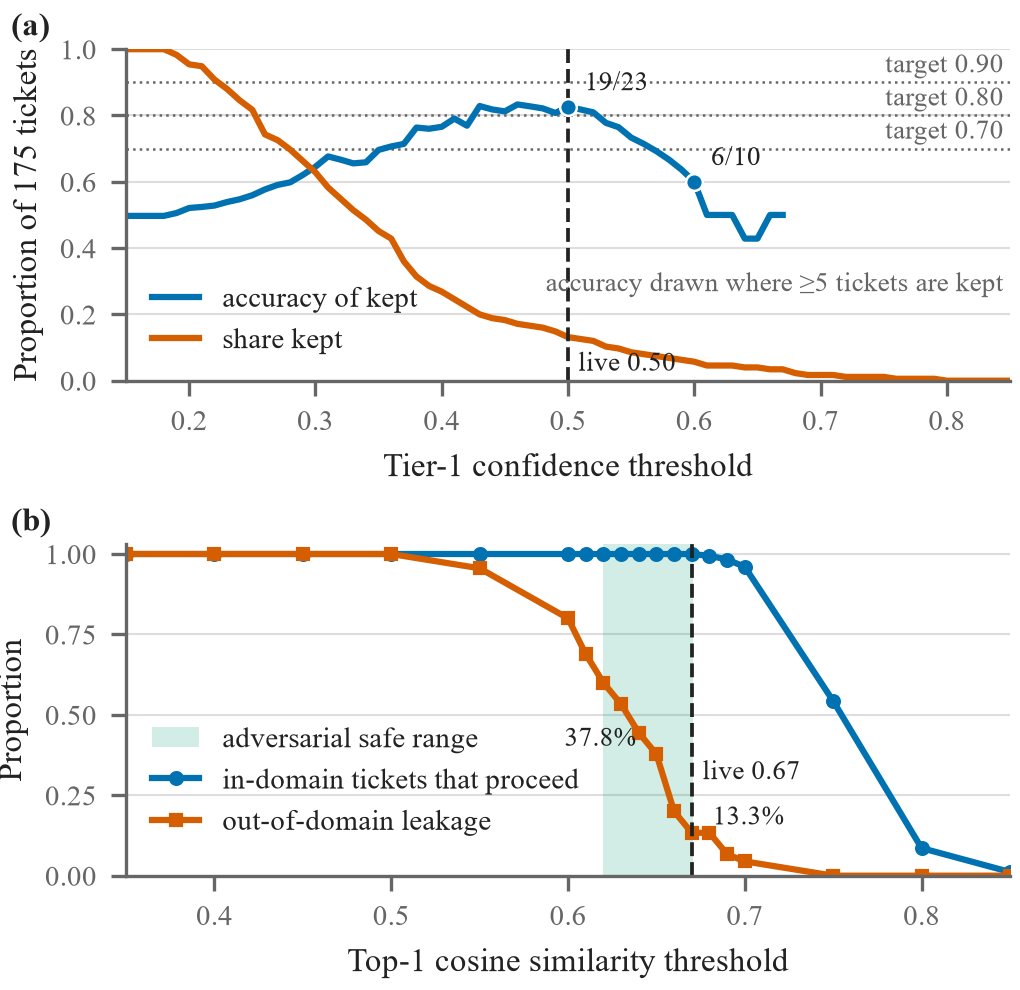
\includegraphics[width=3.05in]{fig2_thresholds.png}
\caption{Threshold calibration. (a) Cascade threshold on paraphrased tickets; the dashed line marks the live threshold of 0.50. (b) Retrieval threshold sweep; the shaded band is the adversarial safe range [0.6196, 0.6704], and the dashed line marks the live threshold of 0.67.}\label{fig:thr}
\end{figure}

\begin{table}[!t]
\caption{The two gates at their live operating points. Leakage is the share of out-of-domain calibration tickets that clear the retrieval gate}\label{tab:gates}
\centering
\footnotesize
\setlength{\tabcolsep}{3pt}
\begin{tabular}{|P{0.740}|P{0.260}|}
\hline
\textbf{Quantity} & \textbf{Value}\\ \hline\hline
\multicolumn{2}{|l|}{\textit{Retrieval gate}}\\ \hline
Threshold on top-1 cosine similarity & 0.67\\ \hline
In-domain tickets that proceed at the gate & 175/175\\ \hline
Out-of-domain leakage at the gate & 13.3\%\\ \hline
Out-of-domain leakage two steps below & 37.8\%\\ \hline
Adversarial safe range & [0.6196, 0.6704]\\ \hline
Adversarial decided correctly, with gate & 9/9\\ \hline
Adversarial decided correctly, gate removed & 3/9\\ \hline
\multicolumn{2}{|l|}{\textit{Cascade gate}}\\ \hline
Threshold on Tier-1 top-class probability & 0.50\\ \hline
Tier-1 median latency (ms) & 1.04\\ \hline
Tier-2 median latency (ms) & 156.4\\ \hline
Tier-2 cost relative to Tier-1 & 151.0$\times$\\ \hline
\end{tabular}
\end{table}

\section{Results}\label{sec:res}

\subsection{Coverage transfer and the calibration distribution}\label{sec:cov}

Split-conformal coverage on the 45-ticket benchmark (Table~\ref{tab:cov}) gives three linked statements.

\begin{itemize}
\item On our corpus, coverage transfers for the BGE representation but not for the lexical one: at $\alpha$ = 0.10 the gap is $-$0.233 for Tier 1 and $-$0.011 for Tier 2, against a noise band of $\pm$0.045 (two standard deviations of a binomial coverage estimate, n = 175).
\item External replication is inconclusive. On an independently generated corpus (not real production data), a version shift left the tiers indistinguishable (0.0009 against $-$0.0072, band $\pm$0.0165), but that is the wrong kind of shift for a vocabulary-level effect, and that corpus shows almost no representation gap (label accuracy 34.8\% against 37.3\%). A paraphrase shift was blocked by our own pre-registered degeneracy rule (domain AUC 0.9972), so the finding has been shown neither to hold nor to fail outside its corpus.
\item Post-hoc, the paraphrase shift cost Tier 1 10.5 accuracy points against 2.4 for Tier 2 (difference-in-differences $-$0.08042, 95\% CI [$-$0.136364, $-$0.020979]); this does not replace the blocked test.
\end{itemize}

Recalibrating on the deployment-distribution set, with nothing else changed, moves the Tier-1 gap from $-$0.233 to $-$0.144 (for Tier 2 the benefit appears as smaller prediction sets), and density-ratio reweighting \cite{b9} is also only a partial repair, so the lexical tier's guarantee cannot be quoted on out-of-template text and conformal prediction remains a measurement, not a gate.

\begin{table}[!t]
\caption{Split-conformal coverage gap on the 45-ticket benchmark. Only the calibration set changes between the two gap columns. The $\pm$2 s.d. column is twice the binomial standard deviation of a coverage estimate at n = 175}\label{tab:cov}
\centering
\footnotesize
\setlength{\tabcolsep}{3pt}
\begin{tabular}{|P{0.090}|P{0.110}|P{0.220}|P{0.230}|P{0.180}|P{0.170}|}
\hline
\textbf{Tier} & \textbf{$\alpha$} & \textbf{Gap, in-domain cal.} & \textbf{Gap, deployment cal.} & \textbf{$\pm$2 s.d.} & \textbf{Set size}\\ \hline\hline
1 & 0.20 & $-$0.200 & $-$0.244 & 0.060 & 2.69\\ \hline
1 & 0.10 & $-$0.233 & $-$0.144 & 0.045 & 3.40\\ \hline
1 & 0.05 & $-$0.106 & $-$0.083 & 0.033 & 5.00\\ \hline
1 & 0.01 & $-$0.012 & $-$0.012 & 0.015 & 6.67\\ \hline
2 & 0.20 & $-$0.044 & 0.000 & 0.060 & 1.11\\ \hline
2 & 0.10 & $-$0.011 & $-$0.011 & 0.045 & 1.82\\ \hline
2 & 0.05 & 0.028 & $-$0.039 & 0.033 & 2.60\\ \hline
2 & 0.01 & 0.010 & $-$0.012 & 0.015 & 4.80\\ \hline
\end{tabular}
\end{table}

\subsection{The cascade saves latency, not accuracy}\label{sec:lat}

Tier 1 alone scores 16/45, 35.6 points below the full pipeline, but that is the BGE-versus-TF-IDF representation gap, not the value of cascading. Against the fair control, Tier 2 answering every ticket (Table~\ref{tab:casc}), the cascade is one ticket worse on each set (32/45 against 33/45, and 131/175 against 132/175; exact McNemar p = 1.000 for both). It buys speed: Tier 2 costs 151.0$\times$ as much as Tier 1 per ticket (156.4 ms against 1.04 ms median), so median latency falls by 8\% on the benchmark and 18\% on the deployment set. A ticket escalated at the retrieval gate makes no language-model call, so drafting is paid only for tickets that pass it.

\begin{table}[!t]
\caption{Cascade against the control that isolates it (Tier 2 answering everything)}\label{tab:casc}
\centering
\footnotesize
\setlength{\tabcolsep}{3pt}
\begin{tabular}{|P{0.180}|P{0.160}|P{0.150}|P{0.170}|P{0.190}|P{0.150}|}
\hline
\textbf{Set} & \textbf{Tier-2 only} & \textbf{Cascade} & \textbf{Tier-2 (ms)} & \textbf{Cascade (ms)} & \textbf{Saving}\\ \hline\hline
Benchmark & 33/45 & 32/45 & 156.4 & 143.5 & 8.2\%\\ \hline
Deployment & 132/175 & 131/175 & 156.4 & 127.9 & 18.2\%\\ \hline
\end{tabular}
\end{table}

\subsection{Zero-shot LLM baselines}\label{sec:zs}

Gemini and Qwen2.5-3B, a 3-billion-parameter open-weight model run on a laptop CPU \cite{b23}, received byte-identical prompts (Fig.~\ref{fig:acc}). Gemini scores 40/45 (95\% CI [0.765, 0.952]), significantly better than Tier 2 at 33/45 (p = 0.039); Qwen2.5-3B scores 34/45 ([0.613, 0.858]), indistinguishable from Tier 2 (p = 1.000), which does not mean better; Qwen2.5-3B against Gemini gives p = 0.070, not significant. As the benchmark was generated with Gemini, Qwen is a partial control for authorship, and Gemini's margin cannot be attributed to capability alone. This is not like-for-like: it measures what a template-generated training set is worth on differently phrased tickets, not whether an LLM outperforms the pipeline, whose contribution is the calibrated escalation neither zero-shot model provides. Among trained classifiers, representation matters more than model family: two other frozen encoders with the same logistic head score 32/45 and 27/45, and a fine-tuned DistilBERT 18/45 and 21/45 in two runs that differ, so we order neither.

\begin{figure}[!t]
\centering
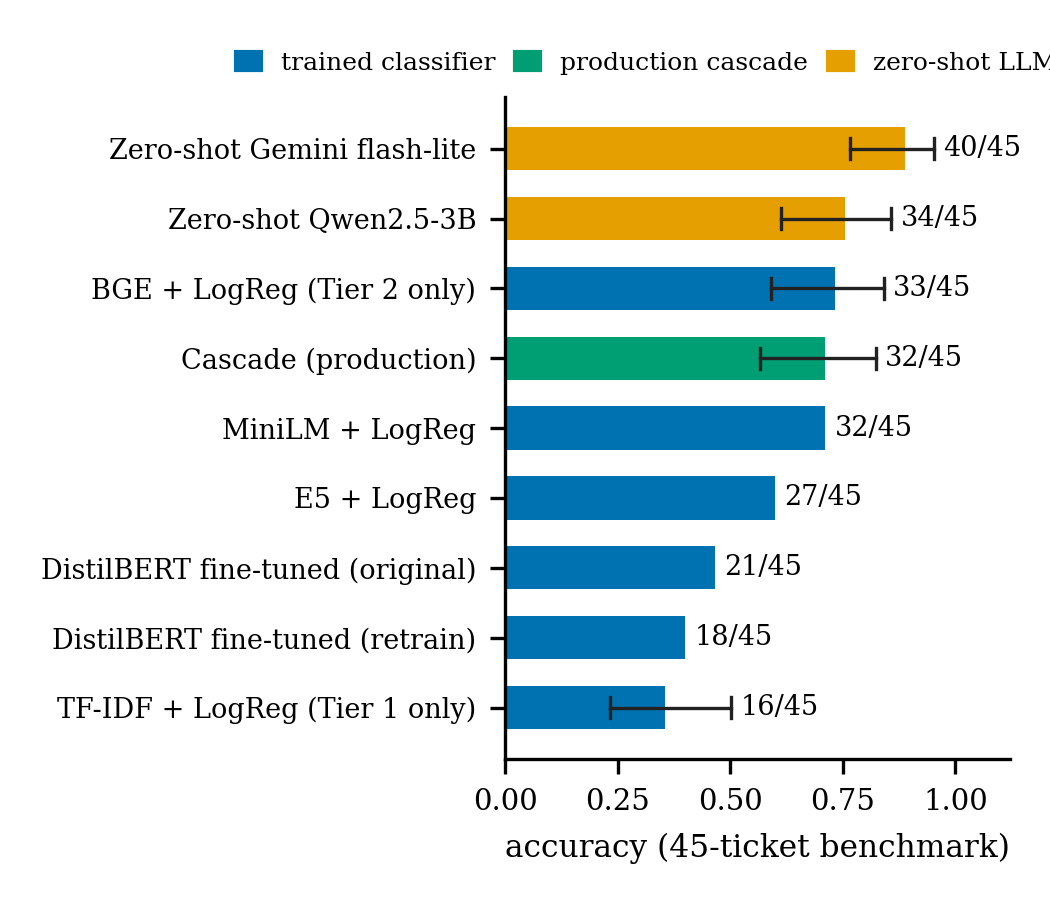
\includegraphics[width=2.55in]{fig3_accuracy.png}
\caption{Accuracy on the 45-ticket out-of-template benchmark. Error bars are Wilson 95\% intervals where the result file records one. Zero-shot models have no abstention mechanism, calibrated gate or cost model.}\label{fig:acc}
\end{figure}

\subsection{Groundedness, an LLM judge, and a sufficiency gate}\label{sec:grd}

All 33 benchmark and adversarial tickets that passed the retrieval gate received a draft, and a human labelled 31/33 as grounded in the retrieved text (95\% CI [0.804, 0.983]). An LLM judge using the same rubric agreed on 30/33 yet reached Cohen's $\kappa$ = $-$0.042 \cite{b24}, every disagreement being the judge rating appropriateness instead of support, so we treat an LLM judge as something to audit, not a way to scale labelling. Future work should check drafts claim by claim against the retrieved text, score entailment with a natural-language-inference (NLI) model, calibrate any automated judge on a small human-labelled set and report judge--human agreement before using it. A retrieval-sufficiency rater that never sees the draft caught 2/2 ungrounded drafts but flagged 26/31 grounded ones, so it cannot be used as a gate.

\subsection{Extended evaluation on independent and real-world tickets}\label{sec:ext}

To test whether these results depend on Gemini-written evaluation text, the unchanged pipeline was run on two more sets (Table~\ref{tab:ext}). Two authors each wrote 54 tickets, seven per category plus five off-topic or vague ones (108 in total), without the training data, templates, benchmarks or LLM assistance, and each labelled the other's tickets blind. Before adjudication Cohen's $\kappa$ was 0.936 for category (bootstrap 95\% CI [0.882, 0.979]; 102/108 agreement) and 1.000 for outcome (108/108); in all 6 adjudicated disagreements the writer's label was kept. The real-world set is the CC BY 4.0 dataset of Pereira \cite{b20}: 2,229 user-typed tickets of an IT-support company, labelled by three IT professionals, of which langid.py \cite{b25} identifies 1,734 as English. A mapping fixed before predictions were examined sends Active Directory and Fileservice (almost entirely file-share access requests) to Access Management and Software and O365 to Application; the other three categories (750 tickets) have no counterpart, so five of our seven teams have no real-ticket evaluation (Section~\ref{sec:lim}). Of the 984 mapped tickets 401 repeat an earlier text exactly, so we report the 583 distinct texts, with all 984 alongside. We found no public, real, English IT ticket dataset whose categories match our seven teams; the Zenodo corpus was the closest real option, and our hand-written set covers all seven.

\begin{table}[!t]
\caption{Results on the independent and real-world test sets (pipeline unchanged)}\label{tab:ext}
\centering
\footnotesize
\setlength{\tabcolsep}{3pt}
\begin{tabular}{|P{0.250}|P{0.090}|P{0.160}|P{0.150}|P{0.200}|P{0.150}|}
\hline
\textbf{Set} & \textbf{n} & \textbf{Cascade acc.} & \textbf{Tier-2 acc.} & \textbf{Escalation rate} & \textbf{Tier-1 share}\\ \hline\hline
Out-of-template (ref.) & 45 & 32/45 & 33/45 & 15/45 (33.3\%) & 4/45\\ \hline
Independent & 108 & 74/98 & 75/98 & 40/108 (37.0\%) & 27/108\\ \hline
Real-world & 583 & 115/583 & 114/583 & 129/583 (22.1\%) & 238/583\\ \hline
\end{tabular}
\end{table}

On the independent set the cascade routes 74 of the 98 tickets that belong to a team correctly (75.5\%, 95\% CI [66.1, 83.0]; Tier 2 alone 75/98), similar to the benchmark's 32/45, with per-team recall from 8/14 (Security) to 14/14 (Database). The gate escalates 40/108 (37.0\% [28.5, 46.4]): 8 of the 10 off-topic or vague tickets, but also 32 of the 98 actionable ones, so the escalate-or-proceed decision is correct for 74/108 (68.5\% [59.3, 76.5]). On real tickets the classifier does not transfer: the cascade routes 115 of 583 distinct texts correctly (19.7\%, 95\% CI [16.7, 23.1]; 119/984, 12.1\%, over all tickets), with recall 86/319 for Access Management and 29/264 for Application, and Tier 2 alone does no better (114/583; exact McNemar p = 1.0). Tier 1 answers 238/583 (40.8\% [36.9, 44.9], against 4/45 on generated text), but only 39 correctly. The gate escalates 129/583 (22.1\% [18.9, 25.7]; 159/984, 16.2\%, over all tickets) but does not filter misroutes: 371 of the 468 misrouted texts still reached the drafter. The alternative mapping changes one assignment, Fileservice to Storage (where our generator files share-permission faults) instead of Access Management, and gives 294/583 (50.4\%, [46.4, 54.5]; online supplement); the escalation rate and Tier-1 share do not depend on the mapping. The jump is a semantic gap between synthetic and real categories: the classifier files real file-share access requests as Storage. The choice of mapping is a sensitivity analysis, not a deployable setting; a production system would need labels in its own categories. A classifier trained only on synthetic templates does not transfer to real tickets, and gates calibrated on the same material do not compensate. The 30 drafts generated for a sample of the real tickets were not labelled.

\textbf{The recurring finding.} The data a component is fitted or calibrated on constrains it more than the method or test applied to it: beyond the coverage gap (Section~\ref{sec:cov}), legitimate deployment-style tickets trigger the in-domain drift reference at rates of 0.217 to 0.646 across four $\alpha$ levels, 3.2 to 38.2 times the per-ticket null, so a monitor on that reference would alarm continuously whatever the test, $\alpha$ or window, and training on the corpus transfers to out-of-template phrasing no better than no training at all (Section~\ref{sec:zs}). Methodological lessons are in the supplement.

\section{Error Analysis}\label{sec:err}

Table~\ref{tab:err} groups the errors of the live pipeline by type.

\begin{table}[!t]
\caption{Error taxonomy of the live pipeline}\label{tab:err}
\centering
\scriptsize
\setlength{\tabcolsep}{3pt}
\begin{tabular}{|P{0.260}|P{0.120}|P{0.620}|}
\hline
\textbf{Error type} & \textbf{Count} & \textbf{Cases and likely cause}\\ \hline\hline
Misclassification (benchmark) & 13/45 & Database$\rightarrow$Application, Infrastructure$\rightarrow$Application and Security$\rightarrow$Storage (2 each); 10 of the 13 errors are wrong predictions of Application or Storage\\ \hline
Safe ticket escalated & 1 & N45: context was adequate but top-1 similarity fell below 0.67\\ \hline
Unsafe ticket drafted & 2 & N26, N31: passed the gate, but the draft was labelled ungrounded\\ \hline
Out-of-domain leakage & 13.3\% & Out-of-domain calibration tickets above 0.67; all 6 are vague `something is broken' messages naming no system (3 of the 15 seeds); no off-topic ticket (weather, food, HR, Finance, Facilities) leaks. Example: `Hey there, something isn't working right on my end and I really need some assistance\ldots{}' (0.725)\\ \hline
Adversarial, gate removed & 6/9 & Off-topic and vague tickets drafted instead of escalated\\ \hline
\end{tabular}
\end{table}

\textbf{Misclassification.} The cascade misroutes 13 of the 45 benchmark tickets (confusion matrix in the online supplement); the most frequent confusions are Database$\rightarrow$Application, Infrastructure$\rightarrow$Application and Security$\rightarrow$Storage (2 each), and 10 of the 13 errors predict Application or Storage. Infrastructure is hardest: recall is 50\% for the trained classifier and for both zero-shot LLMs, which suggests ambiguous wording rather than one weak method. Tier 1 alone misclassifies 29 of 45, mostly where the wording shares no vocabulary with the templates (examples in the supplement).

\textbf{Incorrect escalation decisions.} Of the 13 misclassified benchmark tickets, 5 were escalated (safe) and 8 drafted (unsafe): the classification gate does not stop a misrouted ticket from reaching the drafter, a structural limitation of the current design, seen at scale in 16 of 24 misrouted independent and 371 of 468 misrouted real texts. The retrieval gate cannot catch misrouting by construction: its only input is the top-1 similarity to past tickets of any team, so it checks whether a similar past ticket exists, not whether the predicted team is correct. The gate escalated 97 misrouted and 32 correctly routed real texts, so its similarity does not track routing correctness; nor does Tier-1 confidence (39 of the 238 real texts kept at 0.50 were correct). A cheap consistency check, which we have not tested, would escalate a ticket whose predicted team disagrees with the teams of its top-5 retrieved tickets.

\textbf{Unsupported resolutions.} In both ungrounded drafts the model noted that the retrieved tickets did not match (N26 retrieved fixes for failing disks behind network file shares, N31 NTFS permission fixes), then supplied steps from outside knowledge, which the prompt forbids, and asked for human review; N31 had also been misrouted to Storage. Neither the sufficiency rater nor the LLM judge (Section~\ref{sec:grd}) can yet replace human review.

\section{Limitations}\label{sec:lim}

\textbf{Synthetic data and small evaluation sets.} All training data is synthetic and template-generated, and the evaluation sets are small: at 45 tickets the Wilson interval on Tier 2's 33/45 is [0.590, 0.840] and the conformal noise band at $\alpha$ = 0.10 is $\pm$0.045, so most comparisons between strong methods cannot be ordered. The benchmark and deployment set were written by Gemini, which also drafts resolutions and forms one baseline, and the external transfer corpus is itself generated. The independent set's 108 tickets were written and labelled by two authors who know the categories, so it is small and is not real traffic. The real-world set covers only two of our seven teams, as no public, real, English IT ticket dataset with matching categories was available, so the other five (Database, Infrastructure, Network, Security and Storage) have no real-ticket evaluation. Its accuracy depends strongly on the category mapping (19.7\% or 50.4\%), the tickets come from one organisation, and the English filter let a few non-English tickets through, because their system-generated subject lines were in English.

\textbf{No live evaluation and few human quality labels.} The system has not been deployed: 583 real tickets were routed offline, but no live stream has passed through it and no help-desk user has acted on its output, so its effect on resolution time, misrouting cost and user trust is unmeasured, and the drift monitor has no deployment-traffic reference. Resolution quality rests on human labels for only 33 drafts; an LLM judge could not scale them, its 30/33 raw agreement concealing a Cohen's $\kappa$ of $-$0.042, so the share of grounded drafts is known only within [0.804, 0.983].

\section{Conclusion and Future Work}\label{sec:concl}

Of our two separately calibrated gates, the retrieval gate decides 9/9 adversarial tickets correctly against 3/9 without it, and the cascade cuts median latency by 8\% to 18\% without improving accuracy. These conclusions are established on a synthetic corpus, small LLM-generated evaluation sets, 108 hand-written tickets and 583 real tickets that cover only two of the seven teams, and they should not be read as performance claims for a production help desk. On real tickets the classifier did not transfer (19.7\% routed correctly, 50.4\% under the alternative mapping; 371 of 468 misroutes reached the drafter): the synthetic training data, not the choice of method or threshold, limits what the pipeline can do. Before production use, both thresholds must be recalibrated on the target desk's own tickets.

\textbf{Future work.} Domain adaptation could narrow the synthetic-to-real gap: few-shot fine-tuning on a small labelled set of real tickets, prompt tuning, and self-training on unlabelled real tickets. A real evaluation of all seven teams with a partner IT service desk would replace the two-team test and probe the recurring finding outside our corpus, and hierarchical classification (coarse category first, then team) or zero-shot prompting could handle unseen categories. A shadow deployment, running alongside human triage without acting, would measure resolution time, re-routing rate and cost, and supply the labelled tickets needed to keep the gates current as traffic changes: periodic recalibration on a rolling window of recent labelled tickets, drift monitoring that triggers recalibration, and weighted \cite{b9} or online \cite{b11} conformal methods. More drafts need human labels, for sufficiency as well as support.

\section*{Acknowledgment}
The authors used AI assistants (Anthropic Claude) for code development, experiment scripting and language editing. All experiments were run and checked by the authors, and every reported number is regenerated from committed result files. The independent test tickets were written and labelled by the authors without AI assistance.

\begin{thebibliography}{00}
\bibitem{b1} F.-R. Liu et al., ``TickIt: Leveraging large language models for automated ticket escalation,'' in Proc. 33rd ACM Int. Conf. Foundations of Software Engineering (FSE), 2025.
\bibitem{b2} E. Paket et al., ``IT service desk ticket classification via large language models,'' in Proc. 9th Int. Conf. Computer Science and Engineering (UBMK), 2024.
\bibitem{b3} A. Carroll et al., ``Evaluating large language models for automated REDCap support ticket triage and response,'' JAMIA Open, 2026.
\bibitem{b4} W. Jitkrittum et al., ``When does confidence-based cascade deferral suffice?'' in Advances in Neural Information Processing Systems (NeurIPS), 2023.
\bibitem{b5} Y.-F. Dou et al., ``Conformal cascade: Distribution-free accuracy guarantees for multi-tier LLM inference,'' 2026, arXiv:2607.25018.
\bibitem{b6} C. Fanconi et al., ``Cascaded language models for cost-effective human--AI decision-making,'' in Advances in Neural Information Processing Systems (NeurIPS), 2025.
\bibitem{b7} V. Vovk, A. Gammerman, and G. Shafer, Algorithmic Learning in a Random World. New York: Springer, 2005.
\bibitem{b8} A. N. Angelopoulos and S. Bates, ``Conformal prediction: A gentle introduction,'' Foundations and Trends in Machine Learning, vol. 16, no. 4, pp. 494--591, 2023.
\bibitem{b9} R. J. Tibshirani, R. F. Barber, E. J. Cand\`{e}s, and A. Ramdas, ``Conformal prediction under covariate shift,'' in Advances in Neural Information Processing Systems (NeurIPS), 2019.
\bibitem{b10} R. F. Barber, E. J. Cand\`{e}s, A. Ramdas, and R. J. Tibshirani, ``Conformal prediction beyond exchangeability,'' The Annals of Statistics, vol. 51, no. 2, pp. 816--845, 2023.
\bibitem{b11} I. Gibbs and E. J. Cand\`{e}s, ``Adaptive conformal inference under distribution shift,'' in Advances in Neural Information Processing Systems (NeurIPS), 2021.
\bibitem{b12} P. Lewis et al., ``Retrieval-augmented generation for knowledge-intensive NLP tasks,'' in Advances in Neural Information Processing Systems (NeurIPS), 2020.
\bibitem{b13} H. Joren et al., ``Sufficient context: A new lens on retrieval augmented generation systems,'' in Proc. Int. Conf. Learning Representations (ICLR), 2025.
\bibitem{b14} S.-Q. Yan et al., ``Corrective retrieval augmented generation,'' 2024, arXiv:2401.15884.
\bibitem{b15} J. Jung, F. Brahman, and Y. Choi, ``Trust or escalate: LLM judges with provable guarantees for human agreement,'' in Proc. Int. Conf. Learning Representations (ICLR), 2025.
\bibitem{b16} S. Jain et al., ``Beyond consensus: Mitigating the agreeableness bias in LLM judge evaluations,'' 2025, arXiv preprint.
\bibitem{b17} G. Maheshwari, D. Ivanov, and K. El Haddad, ``Efficacy of synthetic data as a benchmark,'' 2024, arXiv preprint.
\bibitem{b18} S. Xiao et al., ``C-Pack: Packed resources for general Chinese embeddings,'' in Proc. 47th Int. ACM SIGIR Conf. Research and Development in Information Retrieval, 2024.
\bibitem{b19} J. Johnson, M. Douze, and H. J\'{e}gou, ``Billion-scale similarity search with GPUs,'' IEEE Transactions on Big Data, vol. 7, no. 3, pp. 535--547, 2021.
\bibitem{b20} L. S. B. Pereira, ``Classification of IT support tickets,'' Zenodo, Dec. 2022, doi: 10.5281/zenodo.7648117. Dataset, CC BY 4.0.
\bibitem{b21} E. B. Wilson, ``Probable inference, the law of succession, and statistical inference,'' Journal of the American Statistical Association, vol. 22, no. 158, pp. 209--212, 1927.
\bibitem{b22} Q. McNemar, ``Note on the sampling error of the difference between correlated proportions or percentages,'' Psychometrika, vol. 12, no. 2, pp. 153--157, 1947.
\bibitem{b23} Qwen Team, ``Qwen2.5 technical report,'' 2024, arXiv:2412.15115.
\bibitem{b24} J. Cohen, ``A coefficient of agreement for nominal scales,'' Educational and Psychological Measurement, vol. 20, no. 1, pp. 37--46, 1960.
\bibitem{b25} M. Lui and T. Baldwin, ``langid.py: An off-the-shelf language identification tool,'' in Proc. ACL 2012 System Demonstrations, Jeju Island, Korea, 2012, pp. 25--30.
\end{thebibliography}

\end{document}
